\section{Virtual indoor mapping generation workflow}\label{workflow}


\begin{figure*}[ptb] %  figure placement: here, top, bottom, or page
   \centering
   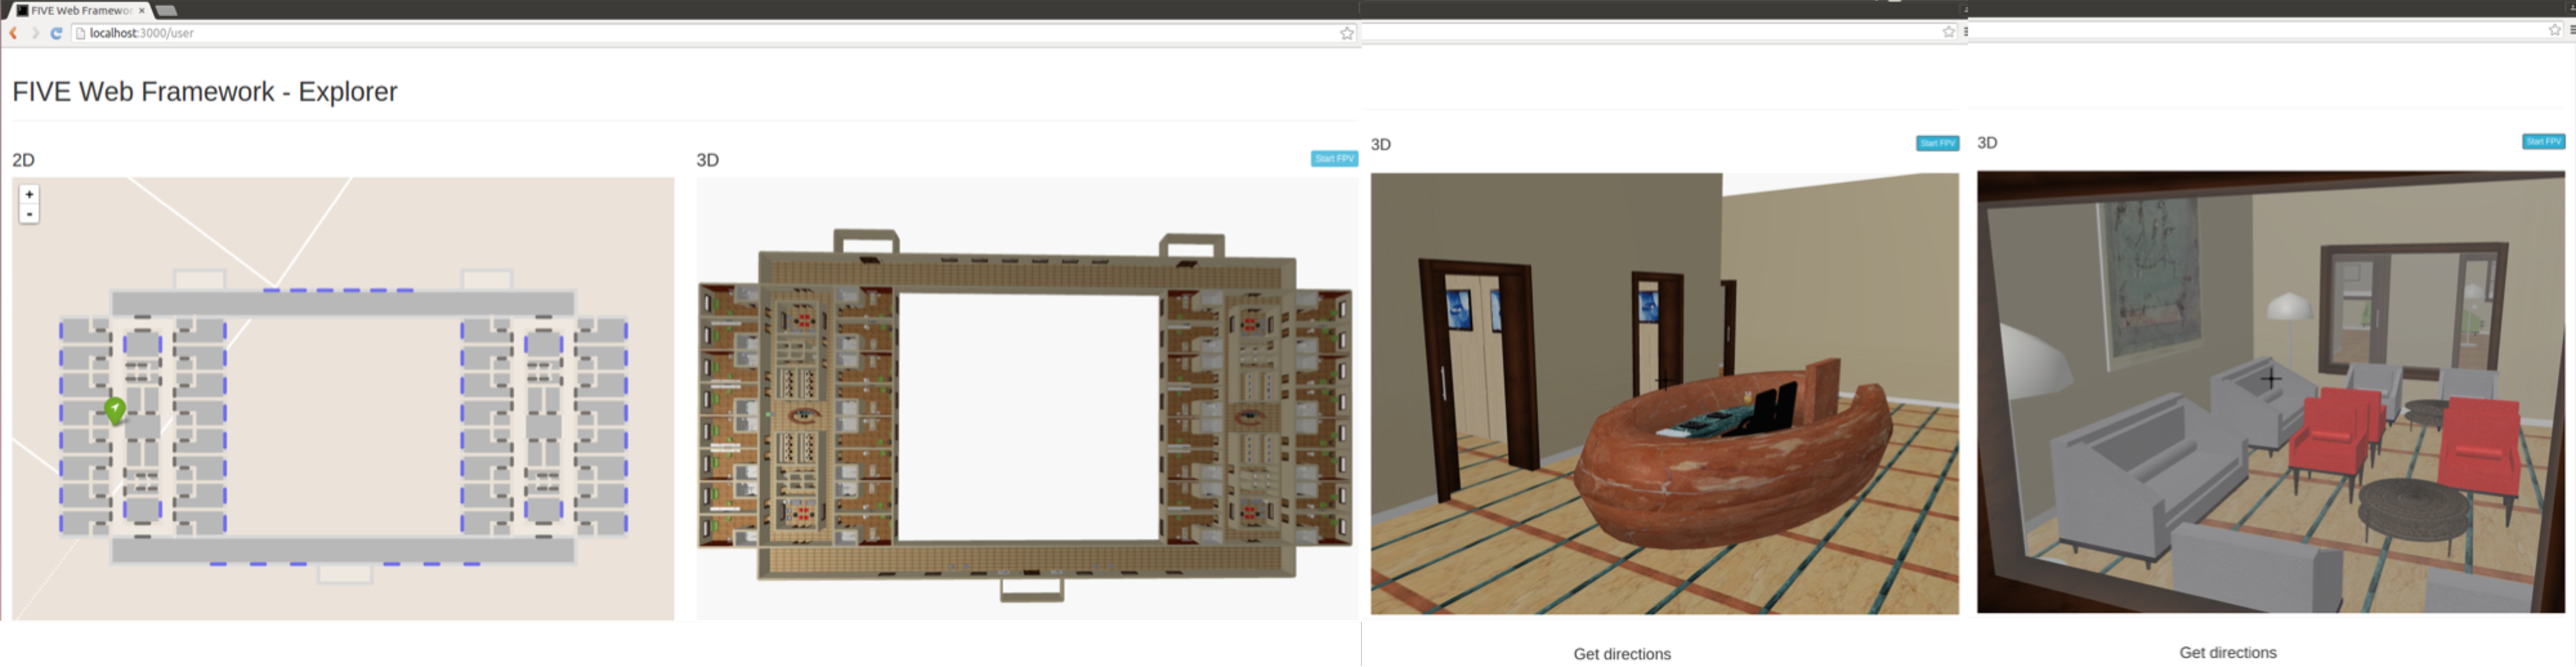
\includegraphics[width=\linewidth]{images/ward/ward} 
   
   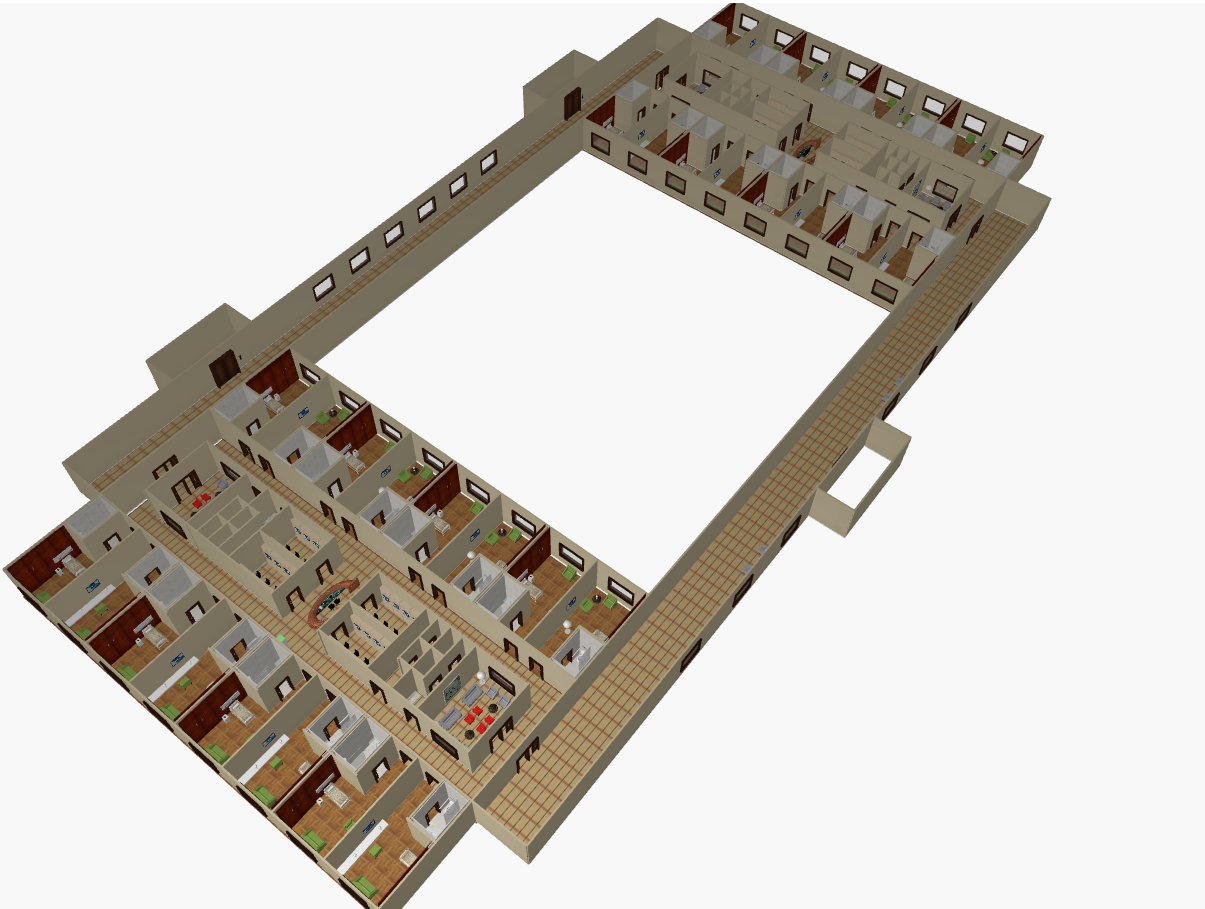
\includegraphics[width=0.327\linewidth]{images/ward/ward1} 
   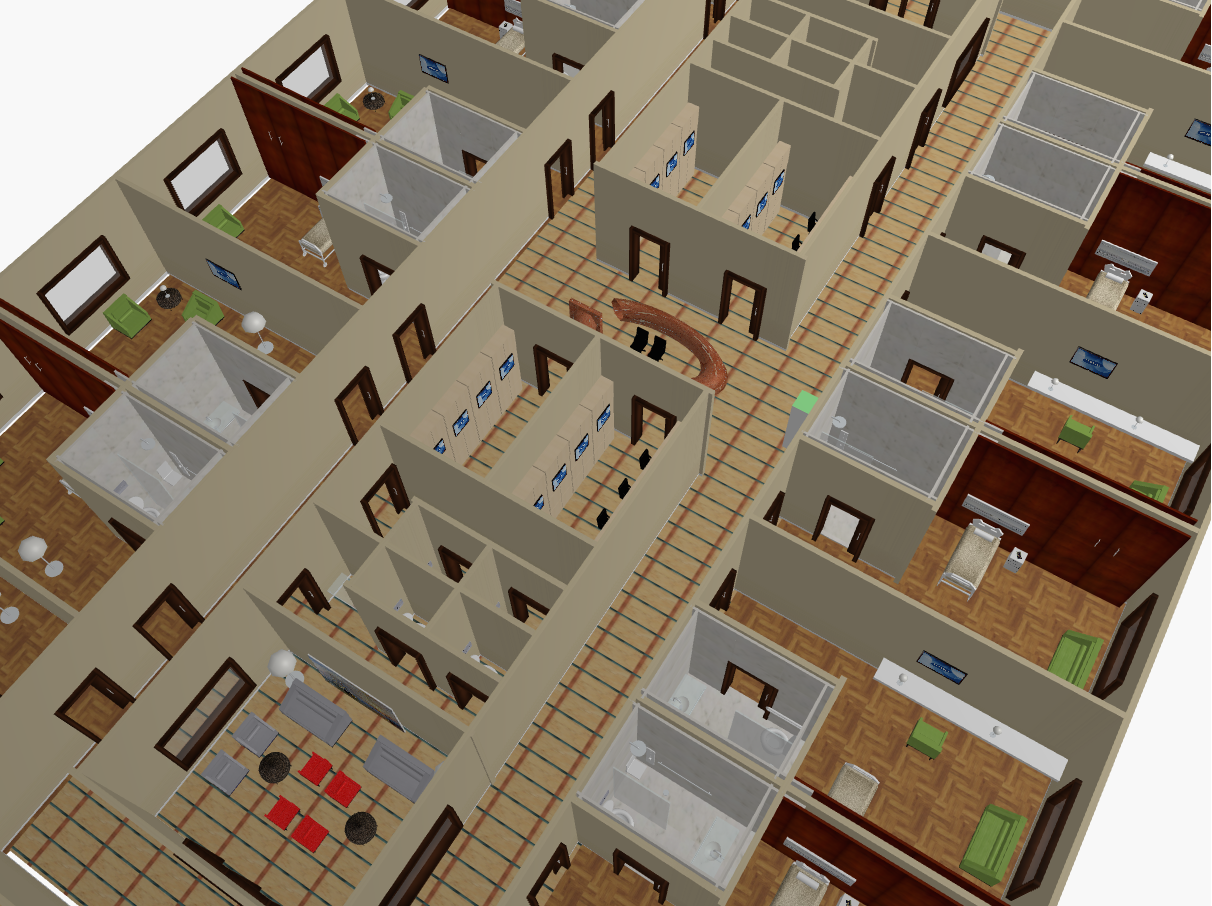
\includegraphics[width=0.327\linewidth]{images/ward/ward4} 
   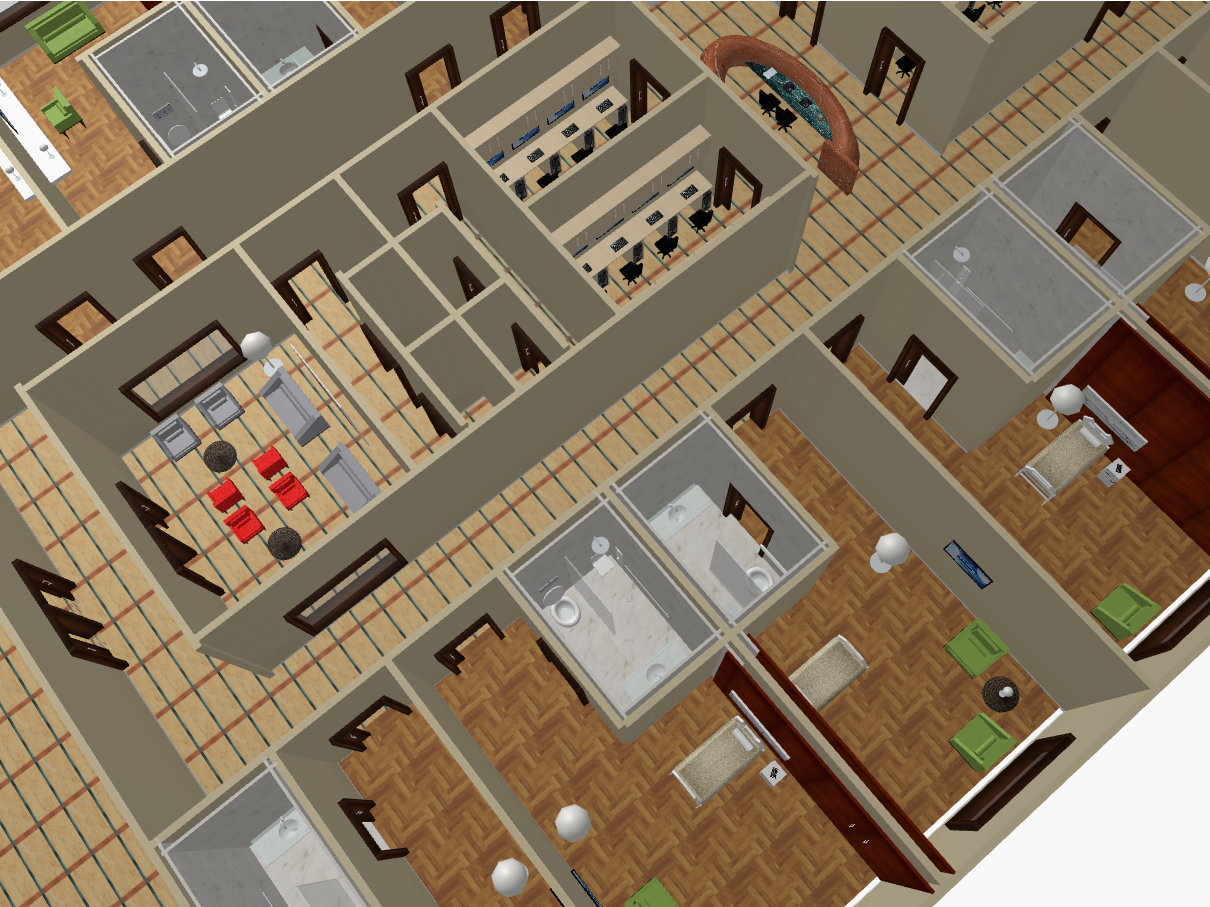
\includegraphics[width=0.327\linewidth]{images/ward/ward5} 
   \caption{example caption}
   \label{fig:example}
\end{figure*}



\begin{figure*}[ptb] %  figure placement: here, top, bottom, or page
   \centering
   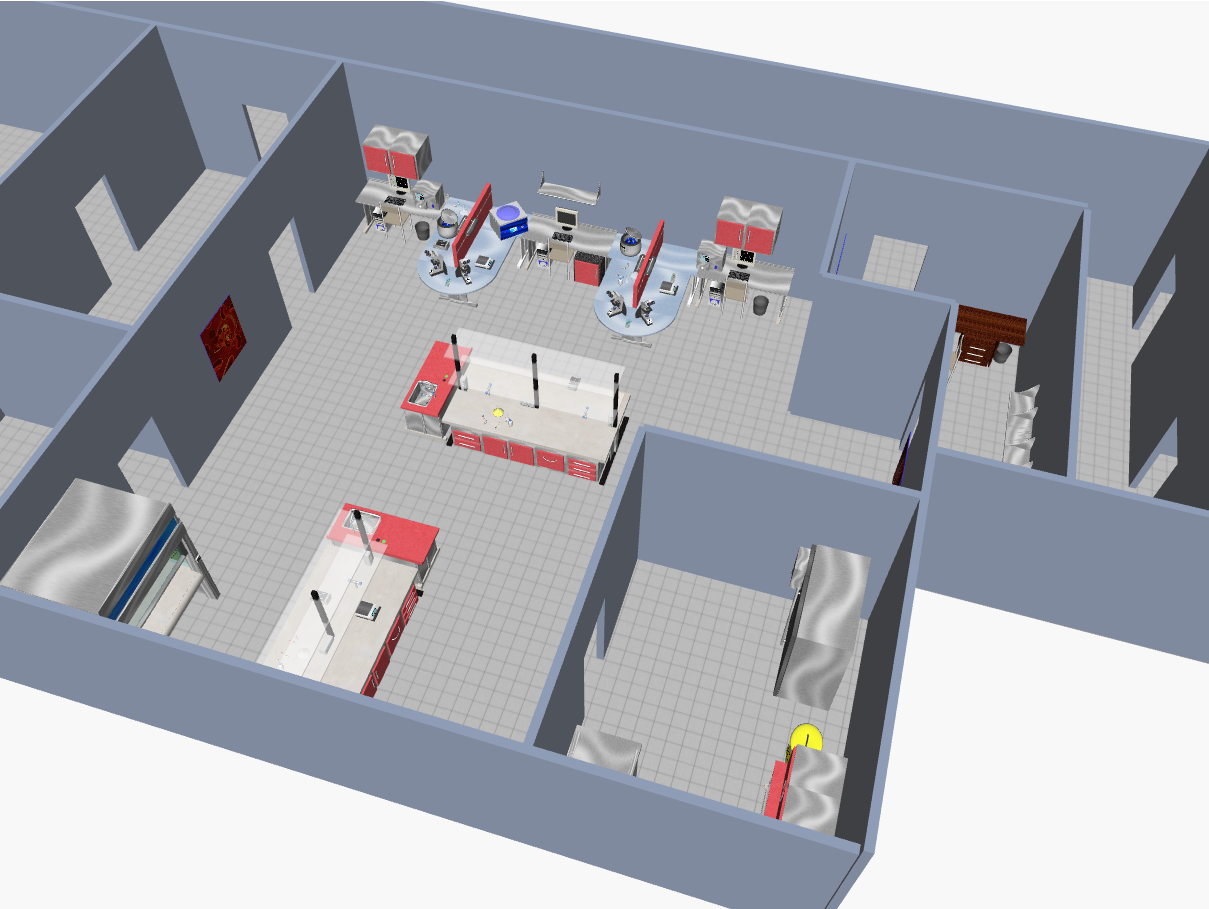
\includegraphics[width=0.327\linewidth]{images/lab/lab0} 
   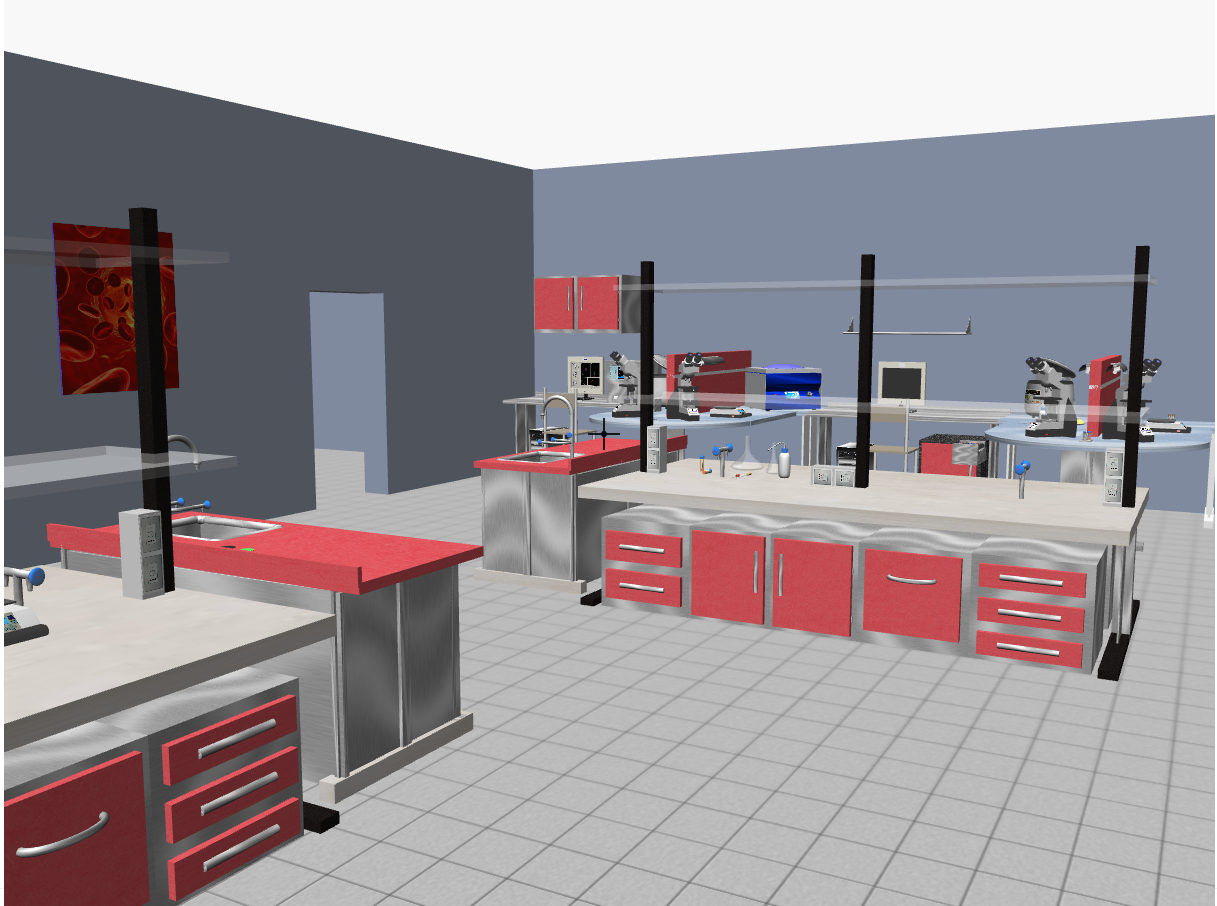
\includegraphics[width=0.327\linewidth]{images/lab/lab2} 
   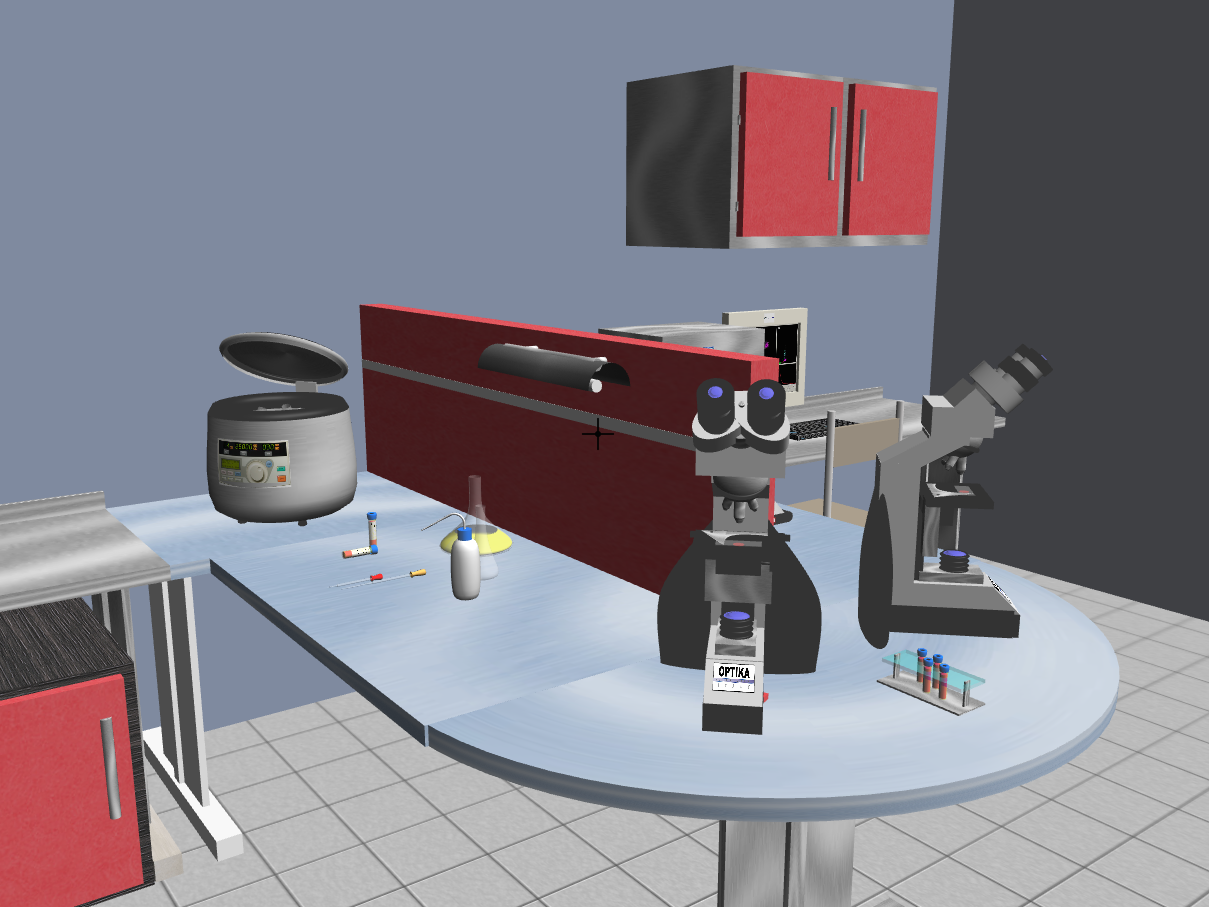
\includegraphics[width=0.327\linewidth]{images/lab/lab3} 

   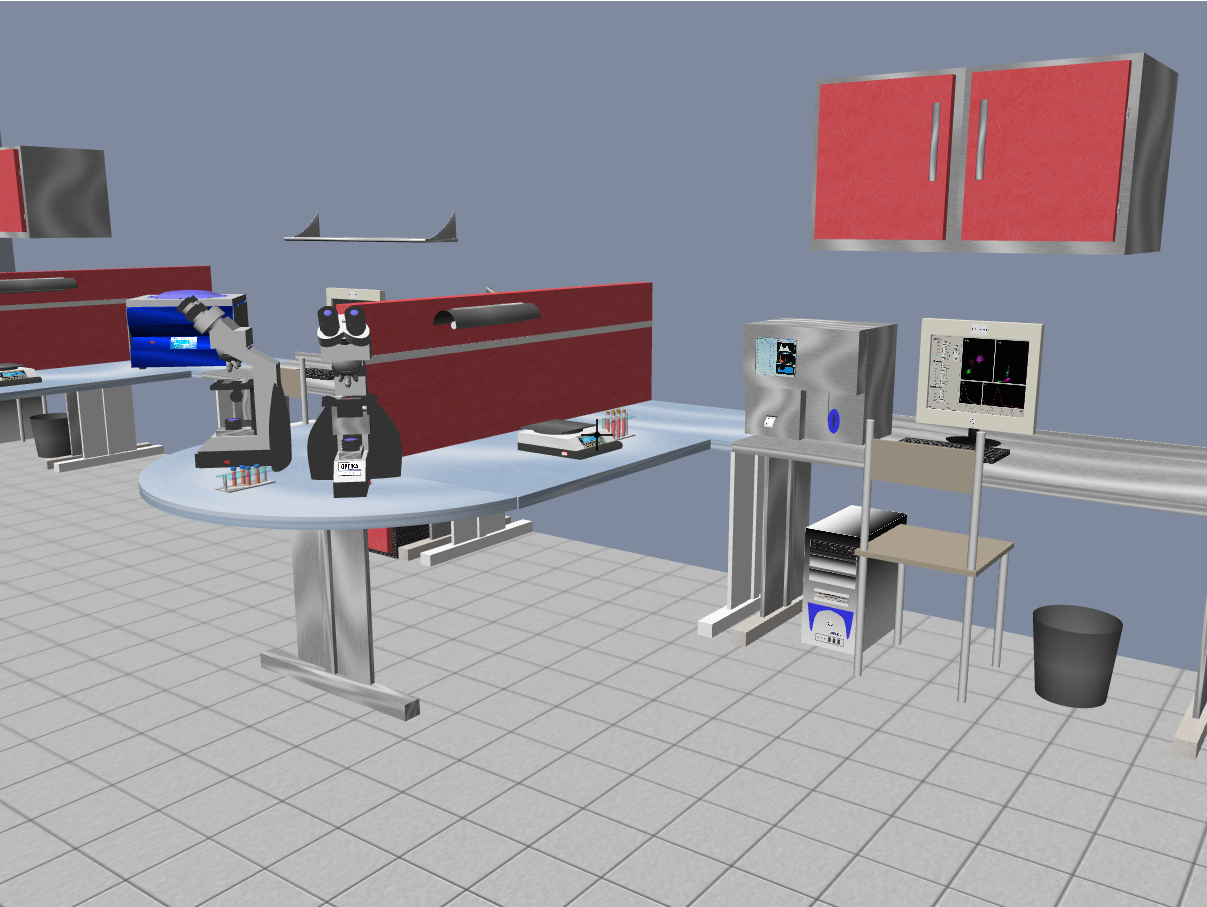
\includegraphics[width=0.327\linewidth]{images/lab/lab4} 
   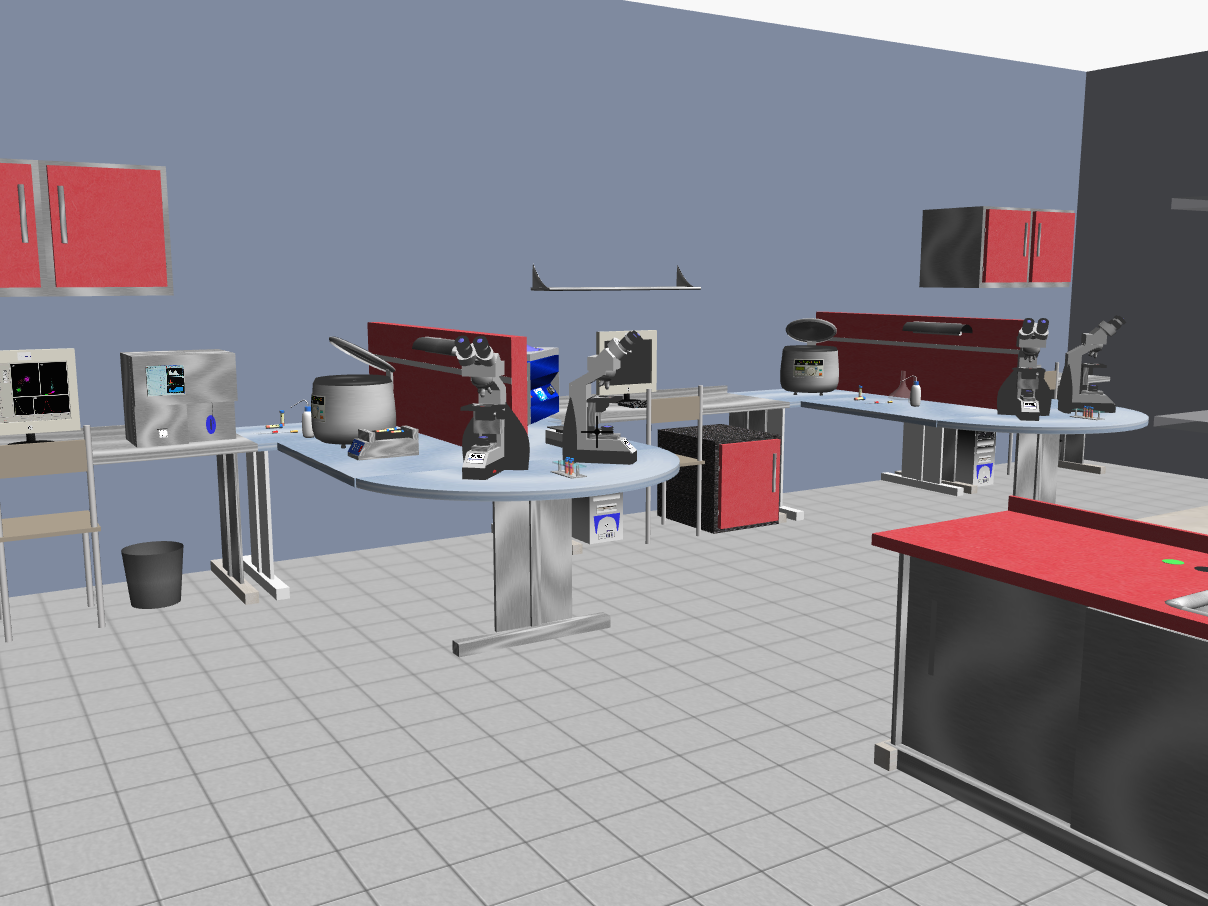
\includegraphics[width=0.327\linewidth]{images/lab/lab5} 
   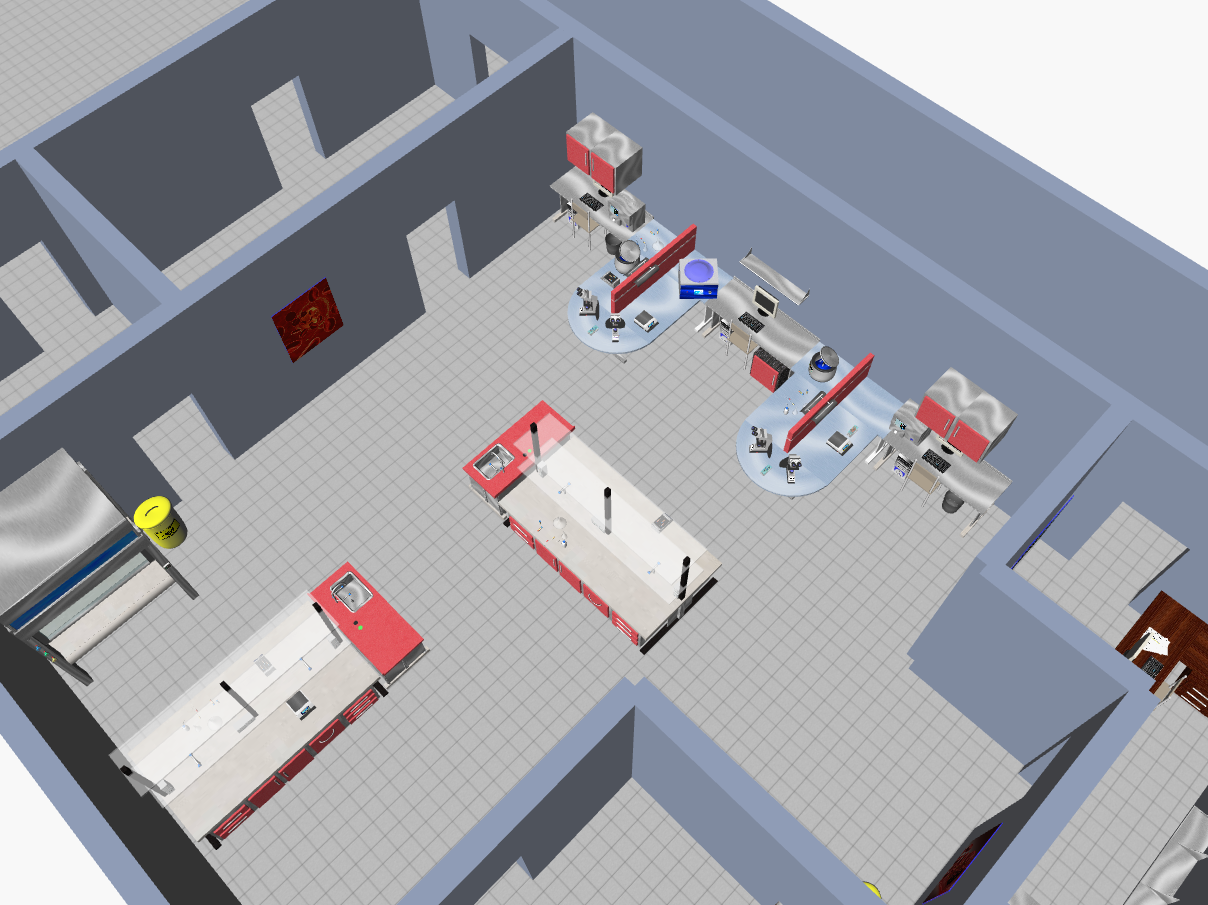
\includegraphics[width=0.327\linewidth]{images/lab/lab6} 
   \caption{example caption}
   \label{fig:example}
\end{figure*}

As case study of the discussed approach, we have taken into account the need of Sogei S.p.A. to support its maintenance service  workflow, since its data center, one of biggest data centers in Europe, is subject to very strict access control policies. 

The overall state of the data center can be monitored through the \emph{Supervisor} client. In this case the considered smart objects belong to a range of different devices, going from webcams, that provide on request the captured video streams, by way of alarm and antifire systems, till to individual servers, that can be monitored along several dimensions, including operating temperature, workload, etc. 

The most common maintenance scenario consists of an intervention by a technician that have to move across the environment, and locate within a huge data center the machine on which to operate, a not trivial task due to the presence of thousands of similar-looking machine racks. Thus the operator will be equipped with an \emph{Explorer} client, which will drive him to the target machine on which operate, while continuously notifying to a security \emph{Supervisor} his position, obtained by interacting with the indoor positioning system.
The maintenance workflow supervisor, using the \emph{Supervisor} client, is able to monitor the operator position within the data center, verifying that he does not deviate on unauthorized paths, triggering some console alarm if this happens.

The purpose is to support  the process of those in charge of carrying out the ``ticket-maintenance'' activities, as quickly  as possible and without error. The ``maintenance man'' will be guided to the right sub-system among thousands of racks. The real-time awareness of the relative positions between the ``maintenance man'' and the rack --- containing the sub-system --- will help to reduce intervention times and to increase safety. By  knowing when the maintenance process starts, the system  can automatically move, in real time, services, which are hosted on virtual machines, to other systems, thus maintaining the continuity of services and, at the same time,  reducing  the global risk factor. When the ``ticket-maint\-enan\-ce'' is over, and the technician goes away, it is possible to immediately  restore  the pre-existing conditions of services after a complete test has been performed.




%----------------------------------------------------------------------------

% right sub­system (inside the rightrack among thousands). We will call them the
% ``maintenance man''. The real­time awareness of the relative positions between
% the ``maintenance man' andthe rack ­ containing the sub­system ­ will help us
% reducing intervention times and increasing safety. If you knew when the
% maintenance process starts, you couldautomatically move,in real time,
% services, that is virtual machines, to other systems,thus
% maintainingcontinuity of services and, in the same time, reducing the
% globalrisk factor. Whenmaintenance is over, and the technician moves away, you
% couldinstantly restore thepre­existing conditions of services, that is,
% immediately after havingperformed an outright test.

% We are now trying to
% verify the possibility to perform a realtime control over the maintenance
% workflow in a complex Data Center. 

% Inparticular, wehave to support the process of those in charge of carrying out
% the ticket­maintenance reaching, as quick as possible and without error, the
% right sub­system (inside the rightrack among thousands). We will call them the
% ``maintenance man''. The real­time awareness of the relative positions between
% the ``maintenance man' andthe rack ­ containing the sub­system ­ will help us
% reducing intervention times and increasing safety. If you knew when the
% maintenance process starts, you couldautomatically move,in real time,
% services, that is virtual machines, to other systems,thus
% maintainingcontinuity of services and, in the same time, reducing the
% globalrisk factor. Whenmaintenance is over, and the technician moves away, you
% couldinstantly restore thepre­existing conditions of services, that is,
% immediately after havingperformed anoutright test.

